\documentclass[11pt]{article}
%you can look for fun LaTeX packages to use hereasdf

\usepackage{amsmath}
\usepackage{amssymb}
\usepackage{fancyhdr}
\usepackage{amsthm}

\usepackage{graphicx}
\usepackage{dcolumn}
\usepackage{bm}

%fun commands for fun sets
%make sure to use these in math mode
\newcommand{\Z}{\mathbb{Z}}
\newcommand{\R}{\mathbb{R}}
\newcommand{\N}{\mathbb{N}}
\newcommand{\C}{\mathbb{C}}
\newcommand{\m}{\mathcal{M}}
\newcommand{\Tt}{\mathcal{T}}
\newcommand{\pa}{\partial}
\newcommand{\dD}{\mathcal{D}}
\newcommand{\E}{\mathbb{E}}



\oddsidemargin0cm
\topmargin-2cm    
\textwidth16.5cm   
\textheight23.5cm  

\newcommand{\question}[2] {\vspace{.25in} \hrule\vspace{0.5em}
\noindent{\bf #1: #2} \vspace{0.5em}
\hrule \vspace{.10in}}
\renewcommand{\part}[1] {\vspace{.10in} {\bf (#1)}}

\newcommand{\myname}{Alex Havrilla}
\newcommand{\myandrew}{alumhavr}
\newcommand{\myhwnum}{Hw 1}

\newtheorem{prop}{Prop}
\newtheorem{lemma}{Lemma}
\newtheorem{theorem}{Theorem}
\theoremstyle{remark}
\newtheorem*{rem}{Remark}
\newtheorem*{defi}{Def}
\newtheorem*{apps}{Application}
\newtheorem*{quest}{Question}
\newtheorem*{ans}{Answer}
\newtheorem*{interest}{Interesting}
\newtheorem*{theme}{Theme}
\newtheorem*{back}{Background}

\setlength{\parindent}{0pt}
\setlength{\parskip}{5pt plus 1pt}
 
\pagestyle{fancyplain}
\lhead{\fancyplain{}{\textbf{HW\myhwnum}}}      % Note the different brackets!
\rhead{\fancyplain{}{\myname\\ \myandrew}}
\chead{\fancyplain{}{\mycourse}}

\title{Type L Easy Regime}

\linespread{1.3}

\begin{document}

\maketitle

We seek to show $(1,1,0,0,...)$ a minimizer and $(\frac{1}{\sqrt{n}},\frac{1}{\sqrt{n}},...)$ a maximizer for the expression

\begin{align*}
	\E|\sqrt{a_1}X_1 + \sqrt{a_2}X_2 + W|^p
\end{align*}

where $X_i \sim \frac{1}{\sqrt{2 \pi }}x^2e^{-x^2/2} = L(x)$

Suppose $a_1 > a_2$. Set $X_{\epsilon} = \sqrt{a_1-\epsilon}X_1 + \sqrt{a_2+\epsilon}X_2$. Wlog  we may suppose $a_1 + a_2 =1$. Then we show

\begin{align*}
	&\E_W \E_X [|X_{\epsilon} + W|^p - |X_0 + W|^p] =\\ 
	&\E_W \int_0^{\infty} [|\sqrt{x}+W|^p+|-\sqrt{x}+W|^p+\alpha x + \beta](f_{\epsilon}(\sqrt{x}) - f_0(\sqrt{x}))\frac{1}{2\sqrt{x}}dx
	 \geq 0
\end{align*}

where $\alpha, \beta$ depend on the densities $f_{\epsilon}$. By known arguments it suffices to show $f_{\epsilon}(\sqrt{x}) - f_0(\sqrt{x})$ has exactly two zeroes(note it must have at least two since $X_{\epsilon}$ have fixed variances and both f are probability distributions).

Fix $a_1 > a_2 \in \R_+$. Compute for arbitrary $a_1,a_2$ the density

\begin{align*}
	f_0(y) = \int_{-\infty}^{\infty} L(x/\sqrt{a_1})L((y-x)/\sqrt{a_2}) dx &= \frac{e^{-y^2/2}}{\sqrt{2\pi}}\frac{3a_1a_2 + (a_1^2-4a_1a_3 + a_2^2)y^2 + a_1a_2y^4}{\sqrt{1/a_1a_2}} \\ 
	&= \frac{e^{-y^2/2}}{\sqrt{2\pi}} ((a_1a_2)^{3/2}(y^4-2y^2+3) + \sqrt{a_1a_2}(a_1-a_2)^2y^2)
\end{align*}

Then considering $g(y) = f_{\epsilon}(\sqrt{y}) - f_0(\sqrt{y})$ we can only be 0 when the polynomial expression $(b_1b_2)^{3/2}(y^4-2y^2+3) + \sqrt{b_1b_2}(b_1-b_2)^2y^2-(a_1a_2)^{3/2}(y^4-2y^2+3) + \sqrt{a_1a_2}(a_1-a_2)^2y^2$ is 0 where $b_1  = a_1 - \epsilon$, and similarly for $b_2$. Then it suffices to show this expression convex. But trivially by taking two derivatives in y we see

\begin{align*}
	g''(y) =  2(b_1b_2)^{3/2}-2(a_1a_2)^{3/2} \geq 0
\end{align*}

since $b_1b_2 = (a_1-\epsilon)(a_2 + \epsilon) \geq a_1a_2$ when $a_1 > a_2$. 

More generally for $b \in [0,1]$ we have if $L_b(x) = (1-b+bx^2)\frac{e^{-x^2/2}}{\sqrt{2 \pi}}$ then 

\begin{align*}
	f_{a,b,0}(x) = e^{-y^2/2}(1-b+3a_1a_2b^2 + b(1-6a_1a_2b)y^2 + a_1a_2 b^2y^4)
\end{align*}

(via mathematica)

so exactly the same analysis carries over since we have the highest order term $a_1a_2b^2y^4$. 

\textbf{The General Case:}

We look at the more general case $\sqrt{a_1}X_{b_1} + \sqrt{a_2}X_{b_2}$ where the $X_c \sim (1-c +cx^2)e^{-x^2/2}$. Mathematica tells us the density of this is 

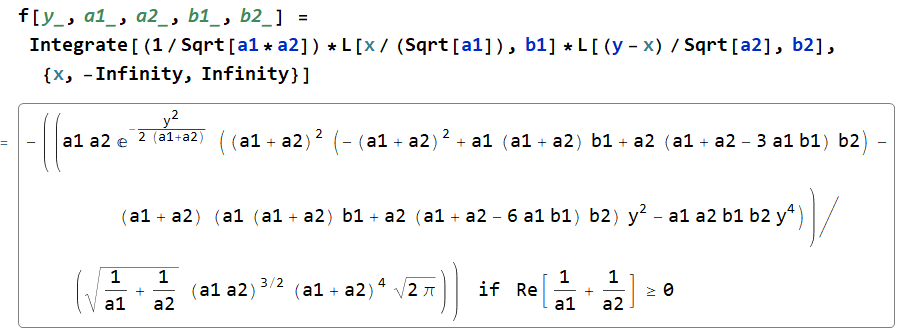
\includegraphics[width=500px]{pics/a_b_parameterization.PNG}

In particular then pay attention to the highest order term $a_1a_2b_1b_2$ which after a quadratic change of variables is $a_1a_2b_1b_2y^2$, a quadratic. Hence $f_{\epsilon} - f_0$ is convex as it is quadratic in terms of $\sqrt{y}$. Note this is true for shifting mass both from $a_1$ to $a_2$ and $b_1$ to $b_2$. 

\textbf{Khintchine Inequalities:} This gives us the usual khintchine type inequalities anytime we have a sum of the form $\sum \sqrt{a_i}X_{b_i}$ for $\sum a_i = 1$, and $X_{b_i}$ a valid gaussian-quadratic polynomial(atomic) type L random variable. Thus this yields khintchine type inequalities for all type L random variables which can be written as linear combinations of the $X_{b_i}$.



\textbf{Structural Thoughts:}


Type L characteristic is of the form $e^{-bx^2/2}\prod_i (1- \alpha_i x^2)$ with $b > 0,\alpha_i > 0$. Note if $b \geq \sum \alpha_i = \alpha$ then we can write 

\begin{align*}
	e^{-bx^2/2}\prod_i (1- \alpha_i x^2) = e^{-(b-\alpha)x^2/2}\prod_i e^{-\alpha_i x^2}(1-\alpha_ix^2)
\end{align*}

which after multiplication by a constant dependent on the product of the $\alpha_i$ can be rewritten as a linear combination of iid. random variables with characteristic $e^{-x^2/2}(1-x^2)$ since $\alpha_i X \sim \alpha_i f_X(x/a)/a$. Having results for $0 < b < 1$ on $(1-bx^2)$ just seems to allow us to absorb more of the gaussian term into the product. So we know the mixture of the gaussian with the product is the same(up to a constant) as another sum with no gaussian component. (Somehow I feel like we should get more mileage controlling b). Ok maybe not entirely fair, we now have khintchine for sums of gaussians and type L random variables. Something to be done with product representations of $e^{x^2} = lim_{n \to \infty} (1+x^2/n)^n$?

Recall if we have a type L random variable its characteristic must have all real roots in +/- pairs. Thus this is a complete characterization of all type L random variables which have density of the form gaussian times polynomial, ie. there can be no type L random variables of this form which are not sums of random variables with gaussian times quadratic densities whose roots sum to less than the variance of the gaussian.

Class of interest:

\begin{align*}
	\{X : \phi_X(z) = e^{-z^2/2}\prod (1-b_iz^2), b_i > 0\}
\end{align*}




\end{document}

